\subsection{Теорема Жордана}
%В этой главе будет почти полное повторение Лекции 3 из \cite{oshemkov}. Если у вас есть какие-то дополнения с учётом нашего лекционного курса, то прошу мне сообщить об этом.
\begin{definition}
    Для любого подмножества $A$ плоскости отношение: «точки $P,Q \in A$ можно соединить непрерывной кривой, лежащей в $A$» является отношением эквивалентности. Соответствующие классы эквивалентности называются \textit{компонентами линейной связности множества $A$}.
\end{definition}

Внезапная вставка! Лично мне кажется, что такое определение удобнее:
\begin{definition}
    Линейно связное подмножество топологического пространства $X$, не содержащееся в отличном от него самого линейно связном подмножестве $X$, называется \textit{линейно связной компонентой $X$}.
\end{definition} 

\begin{definition}
    Функция $f: X \to \R$, заданная на топологическом пространстве, называется \textit{локально постоянной}, если для каждой точки $x \in X$ существует такая окрестность $B$, что $f$ постоянна на $B$.
\end{definition} 

\begin{statement}
    Локально постоянная функция $f: X \to \R$ непрерывна.
\end{statement} 
\begin{proof}
    Для каждой точки $x \in X$ существует такая окрестность $B$, на которой $f$ постоянна, значит, равна $f(x)$. Но это означает, что
    \[\forall x \in X \ \forall \epsilon > 0 \ \exists B: \ f(B) \in (f(x) - \epsilon, f(x) + \epsilon),\]
    что и является определением непрерывности.
\end{proof} 

\begin{statement}
    Пусть локально постоянная функция принимает не более чем счётное число значений. Тогда она постоянна на каждой компоненте.
\end{statement} 
\begin{proof}
    Пусть $x,y$ — произвольные точки из компоненты, то есть существует непрерывная кривая $\gamma: [a,b] \to X$, для которой $x = \gamma(a)$, $y = \gamma(b)$. Так как локально постоянная функция непрерывна по утверждению выше и композиция непрерывных отображений непрерывна, то функция $g(t) = f(\gamma(t))$ также непрерывна. Однако если $g(a) \neq g(b)$, то $g$ принимает все промежуточные значения, которых континуум — противоречие.
\end{proof} 


\begin{theorem}[Жордана для ломаных]
    Замкнутая вложенная ломаная разбивает плоскость на две компоненты связности. %(сюда рисунок №1)
\end{theorem}
\begin{proof}
    %См. \cite{oshemkov}, сам допишу после следующей лекции или на выходных.
    Шаг 1. Число компонент $\leqslant 2$.

    Чтобы доказать, что число компонент, на которые замкнутая вложенная ломаная разбивает плоскость, не больше двух, достаточно выбрать нужным образом две точки и доказать, что любую точку плоскости можно соединить с одной из них непрерывной кривой, не пересекающей ломаную.

    Выберем на произвольном ребре ломаной точку и рассмотрим круг с центром в этой точке (достаточно малый, чтобы он пересекался только с внутренними точками ребра и не пересекался с другими рёбрами ломаной). Ребро разбивает круг на две части, в каждой из частей выберем по точке (обозначим их $A$ и $B$).

    \begin{figure}[h]
        \centering
        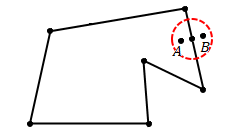
\includegraphics{images/c4.1.png}
        \caption{Круг с центром в точке ломаной.}
        \label{fig:c4.1}
    \end{figure}

    Теперь определим понятие «идти вдоль кривой». Произвольные кривые могут быть устроены достаточно сложно, и для них определить это понятие довольно затруднительно. Для ломаной с конечным количеством звеньев это не вызывает проблем.

    Для произвольной точки $Q$ на ломаной выберем достаточно маленький круг $D_Q$ (т.е. если $Q$ — точка на ребре, то $D_Q$ пересекается только с внутренними точками ребра, если $Q$ — вершина, то $D_Q$ не пересекается с другими рёбрами, кроме двух, выходящих из неё). В каждом таком круге выберем пару точек, лежащих в разных компонентах относительно пары радиусов, на которые они этот круг разбивают. Здесь пользуемся следующей леммой:

    \begin{lemma}
        Два радиуса разбивают круг на две компоненты.
    \end{lemma}
    \begin{proof}
        Пусть $D = \{ (x,y) \in \mathbb{R}^2 \mid x^2 + y^2 \leq R^2 \}$ — замкнутый круг радиуса $R$, и пусть $r_1, r_2$ — два различных радиуса этого круга, исходящие из центра $O$. Обозначим $D^* = D \setminus (r_1 \cup r_2)$. Требуется доказать, что $D^*$ имеет ровно две компоненты линейной связности.

        \begin{figure}[h]
            \centering
            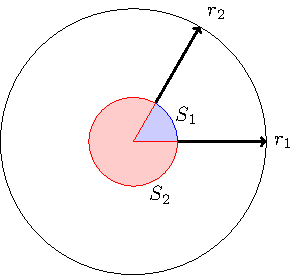
\includegraphics[scale=1]{images/c4.7.pdf}
            \caption{К лемме о разбиении круга на две компоненты.}
            \label{fig:c4.7}
        \end{figure}

        Пусть радиусы заданы углами $\theta_1$ и $\theta_2$ ($\theta_1 \neq \theta_2$). Они делят круг на два открытых сектора:
        \begin{align*}
            S_1 &= \{ (r,\theta) \mid 0 < r \leq R, \theta_1 < \theta < \theta_2 \}, \\
            S_2 &= \{ (r,\theta) \mid 0 < r \leq R, \theta_2 < \theta < \theta_1 + 2\pi \}.
        \end{align*}

        Каждый сектор $S_i$ линейно связен.
        Любое связное множество, содержащее $S_i$, должно пересекать $r_1$ или $r_2$, но $r_1, r_2 \notin D^*$. Следовательно, $S_1$ и $S_2$ — максимальные связные подмножества в $D^*$.

        Все точки $D^*$ принадлежат либо $S_1$, либо $S_2$, а центр $O$ удалён. Таким образом, $D^* = S_1 \sqcup S_2$, где $S_1$ и $S_2$ — две компоненты линейной связности.
    \end{proof}

    Рассмотрим круг, соответствующий вершине, и круг, соответствующий внутренней точке ребра. Несложно понять, что можно выбрать в каждом из кругов пару точек, лежащих в разных частях круга, таким образом, что их можно попарно соединить друг с другом, не пересекая ломаную (выбираем точки достаточно близко к ребру и идём вдоль этого ребра — см.рис.\ref{fig:c4.2}).

    \begin{figure}[h]
        \centering
        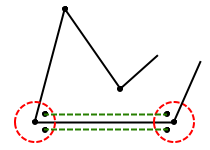
\includegraphics{images/c4.2.png}
        \caption{Проход вдоль ребра.}
        \label{fig:c4.2}
    \end{figure}

    Это означает, что если мы сможем соединить произвольную точку $P$ плоскости с одной из точек любого из кругов, соответствующих точкам ломаной, то мы сможем дальше пройти вдоль ломаной (не пересекая её), и соединить полученную точку либо с точкой $A$, либо с точкой $B$ — см.рис.\ref{fig:c4.3}.

    \begin{figure}[h]
        \centering
        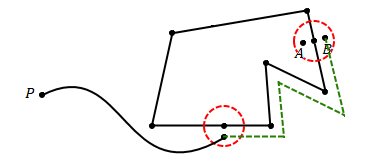
\includegraphics{images/c4.3.png}
        \caption{Проход вдоль ломаной.}
        \label{fig:c4.3}
    \end{figure}

    Осталось понять, что точку $P$ можно соединить с какой-то точкой из какого-то круга с центром на ломаной.
    Выберем произвольную точку $R$ на ломаной и соединим её с точкой $P$ отрезком. $PR$ — непрерывная кривая, значит, существует первая точка $R'$ пересечения этой кривой с ломаной (по лемме о первой точке). Рассмотрим круг $D_{R'}$ и на отрезке $PR'$ отступим от точки $R'$ на расстояние $\epsilon$, меньшее радиуса круга. Из получившейся точки мы можем пойти вдоль ломаной и прийти либо в точку $A$, либо в точку $B$ — см.рис.\ref{fig:c4.4}.

    \begin{figure}[h]
        \centering
        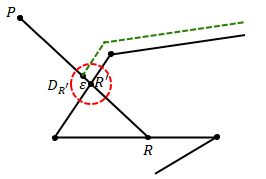
\includegraphics{images/c4.4.png}
        \caption{Соединение произвольной точки плоскости с точкой из круга с центром на ломаной.}
        \label{fig:c4.4}
    \end{figure}

    Таким образом, мы доказали, что количество частей, на которые замкнутая ломаная разбивает плоскость, не может быть больше двух. Чтобы доказать, что таких компонент ровно две, осталось понять, что точки $A$ и $B$, которые мы выбрали, лежат действительно в разных компонентах, то есть, не существует кривой, которая, не пересекая ломаную, соединяет точки $A$ и $B$.

    Шаг 2. Докажем, что число компонент $\geqslant$ 2 (есть точки, лежащие в разных компонентах).

    Рассмотрим ломаную $L$ и точку $P \notin L$. Возможные варианты пересечения (маленькая окрестность точки пересечения) луча $l_P$ с началом в точке $P$ с ломаной $L$ указаны на рисунке \ref{fig:c4.5}.

    \begin{figure}[h]
        \centering
        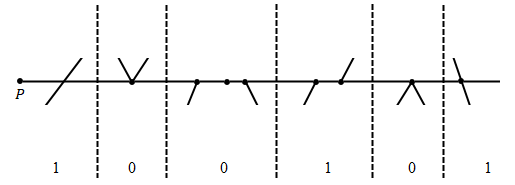
\includegraphics[scale=0.9]{images/c4.5.png}
        \caption{Возможные варианты пересечения $l_P$ с ломаной $L$.}
        \label{fig:c4.5}
    \end{figure}

    Построим инвариант (грубо говоря, посчитаем чётность количества пересечений луча $l_P$ с ломаной $L$, но в случае, когда $l_P$ идёт по ребру $L$, мы получим бесконечное множество точек пересечения, поэтому лучше сказать, что каждому типу пересечения поставим в соответствие 0 или 1, как показано на рисунке \ref{fig:c4.5}).

    Лучу $l_P$ поставим в соответствие число, которое равно сумме по модулю 2 чисел, соответствующих вариантам пересечения этого луча с ломаной $L$:
    $\sigma(l_P)$ — сумма чисел, приписанных пересечением по модулю 2.

    \begin{statement}
        $\sigma(l_P)$ не зависит от луча $l_P$, а только от точки $P$.
    \end{statement} 
    \begin{proof}
        При повороте на малый угол $\phi$ вокруг точки $P$ число $\sigma(l_P)$ не меняется (см.рис.\ref{fig:c4.6}), поэтому функция $\sigma(l_P)$ локально постоянна (если рассматривать её как функцию от $\phi$).

        Однако любая локально постоянная функция на отрезке постоянна.

        \begin{figure}[htbp]
            \centering
            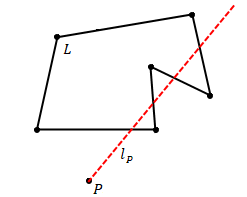
\includegraphics[scale=1]{images/c4.6.png}
            \caption{Подсчёт пересечений луча $l_P$ с ломаной $L$.}
            \label{fig:c4.6}
        \end{figure}
    \end{proof} 

    Таким образом, мы построили функцию $\sigma(P)$ на $\R^2 \setminus L$. Эта функция $\sigma(P)$ тоже локально постоянна, то есть, для любой точки $P \in \R^2 \setminus L$ существует её окрестность $U$ такая, что $\sigma|_U \equiv const$. Значит, функция $\sigma$ постоянна на каждой компоненте множества $\R^2 \setminus L$.

    Действительно, пусть $\gamma: [a,b] \to \R^2 \setminus L$ — произвольная непрерывная кривая, не пересекающая ломаную $L$. Покажем, что значения функции $\sigma$ в точках $\gamma(a), \gamma(b)$ совпадают (это и будет означать, что функция $\sigma$ постоянна на каждой компоненте множества $\R^2 \setminus L$).

    Поскольку кривая $\gamma$ непрерывна, то (по определению непрерывности) для любого $t \in [a,b]$ верно следующее: какую бы окрестность $W$ точки $\gamma(t)$ мы ни выбрали, существует интервал $(t - \epsilon, t + \epsilon)$ такой, что при отображении $\gamma$ этот интервал целиком попадает в эту окрестность (см.рис.\ref{fig:c4.8}).

    \begin{figure}[htbp]
        \centering
        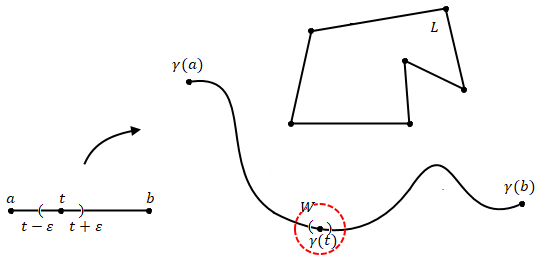
\includegraphics[scale=0.8]{images/c4.8.png}
        \caption{Значения функции $\sigma$ в точках $\gamma(a), \gamma(b)$ совпадают.}
        \label{fig:c4.8}
    \end{figure}

    Рассмотрим $f(t)$ — функцию на отрезке $[a,b]$, определяемую равенством 
    \[f(t) = \sigma(\gamma(t)).\]

    $f(t)$ локально постоянна (так как значение функции $\sigma$ в некоторой окрестности точки $P$ постоянно — мы можем вращать луч $l_P$, а также можем начало луча $l_P$ сдвигать вдоль прямой, содержащей луч — при обеих этих операциях функция $\sigma(P)$ не меняется — действуя таким образом, мы заметём некоторую окрестность точки $P$ на плоскости), поэтому $f(t)$ постоянна на $[a,b]$.

    Это означает, что $f(a) = f(b)$, то есть, $\sigma(\gamma(a)) = \sigma(\gamma(b))$.

    %$\sigma(P)$ — сумма чисел, приписанных пересечением по модулю 2.
    % \begin{lemma}[1]
    %     При фиксированном $X$ функция $\sigma(x, \phi)$ не зависит от $\phi$
    % \end{lemma}
    % \begin{lemma}[2]
    %     Функция $\sigma(x) := \sigma(x, \phi)$ локально постоянна (по $x$).
    % \end{lemma}
    % \begin{proof}
    %     Смотри рисунок (которого нет).
    % \end{proof}
    % \begin{lemma}[3]
    %     $x,y \in \R^2 \setminus L$, $x$ и $y$ можно соединить непрерывной кривой, не пересекающей ломаную.
    % \end{lemma}
    % \begin{proof}
    %     $\exists \gamma: [0,1] \to \R^2 \setminus L$ — непрерывная. $\gamma(0) = x, \ \gamma(1) = y \Rightarrow \sigma(x) = \sigma(y)$.
    % \end{proof}
    % $\gamma([0,1])$ — компактное подмножество плоскости. Т.к. оно связное, то на нём функция $\sigma(x) = const$.

    Итак, мы построили некоторую функцию $\sigma$, которая постоянна на каждой компоненте линейной связности. Чтобы доказать, что число компонент, на которые ломаная делит плоскость, не меньше двух, достаточно предъявить две точки, в которых значения этой функции будут разными.

    Рассмотрим маленький отрезок $P_1 P_2$, перпендикулярный ребру ломаной, и не пересекающий другие рёбра. Луч с началом в точке $P_1$ пересекает ломаную ровно на один раз больше, чем луч с началом в точке $P_2$, поэтому $\sigma(P_1) \neq \sigma(P_2)$. Отсюда следует, что число компонент, на которые замкнутая ломаная разбивает плоскость, не меньше двух.
\end{proof}
